%%%%%%%%%%%%%%%%%%%%%%%%%%%%%%%%%%%%%%%%%%%%%%%%%%%%%%%%%%%%%%%%%%%%%
%
% CSCI 1430 Written Question Template
%
% This is a LaTeX document. LaTeX is a markup language for producing documents. 
% You will fill out this document, compile it into a PDF document, then upload the PDF to Gradescope. 
%
% To compile into a PDF on department machines:
% > pdflatex thisfile.tex
%
% If you do not have LaTeX, your options are:
% - VSCode extension: https://marketplace.visualstudio.com/items?itemName=James-Yu.latex-workshop
% - Online Tool: https://www.overleaf.com/ - most LaTeX packages are pre-installed here (e.g., \usepackage{}).
% - Personal laptops (all common OS): http://www.latex-project.org/get/ 
%
% If you need help with LaTeX, please come to office hours.
% Or, there is plenty of help online:
% https://en.wikibooks.org/wiki/LaTeX
%
% Good luck!
% James and the 1430 staff
%
%%%%%%%%%%%%%%%%%%%%%%%%%%%%%%%%%%%%%%%%%%%%%%%%%%%%%%%%%%%%%%%%%%%%%

% How to include two graphics on the same line:
%
% \includegraphics[width=0.49\linewidth]{yourgraphic1.png}
% \includegraphics[width=0.49\linewidth]{yourgraphic2.png}
%
% How to include equations:
%
% \begin{equation}
% y = mx+c
% \end{equation}
%
%%%%%%%%%%%%%%%%%%%%%%%%%%%%%%%%%%%%%%%%%%%%%%%%%%%%%%%%%%%%%%%%%%%%%%%%%%%%%%%%%%%%%%%%%%%%%%%%

\documentclass[11pt]{article}

\usepackage[english]{babel}
\usepackage[utf8]{inputenc}
\usepackage{amssymb}
\usepackage{xcolor}
\usepackage[colorlinks = true,
            linkcolor = blue,
            urlcolor  = blue]{hyperref}
\usepackage[a4paper,margin=1.5in]{geometry}
\usepackage{stackengine,graphicx}
\usepackage{fancyhdr}
\setlength{\headheight}{15pt}
\usepackage{microtype}
\usepackage{times}
\usepackage[shortlabels]{enumitem}
\setlist[enumerate]{topsep=0pt}
\usepackage{amsmath}
\usepackage{caption}
\usepackage{graphicx}
\usepackage{caption}
\usepackage{subcaption}
\usepackage{minted}
% a great python code format: https://github.com/olivierverdier/python-latex-highlighting
\usepackage{pythonhighlight}

\usepackage{float}
\usepackage{fourier}
\newcommand{\srinath}[1]{\textcolor{orange}{[Srinath: #1]}}

\frenchspacing
\setlength{\parindent}{0cm} % Default is 15pt.
\setlength{\parskip}{0.3cm plus1mm minus1mm}

\pagestyle{fancy}
\fancyhf{}
\lhead{Robot Exercises}
\rhead{CSCI 2952-O}
% \lfoot{\textcolor{red}{Only
% \ifcase\thepage
% \or instructions
% \or A1
% \or A2
% \or Q3
% \or A3
% \or A4
% \or A5
% \or instructions
% \or instructions
% \or A6 
% \or instructions
% \or A7 
% \or feedback
% \else
% EXTRA PAGE ADDED
% \fi
% should be on this page
% }}
% \rfoot{\thepage~/ 13}


\date{}

\title{\vspace{-1cm}52-O: Robot Exercises}


\begin{document}
\maketitle
\vspace{-3cm}
\thispagestyle{fancy}

\section*{Instructions}
\begin{itemize}
  \item 5 robot exercises.
  \item Include code, images, and equations where appropriate.
%   \item Please make this document anonymous.
  \item When you are finished, compile this document to a PDF and submit it directly to Gradescope. 
  \item This assignment is \textbf{fixed length}, and the pages have been assigned for you in Gradescope. As a result, \textbf{please do NOT add any new pages}. We will provide ample room for you to answer the questions. If you \emph{really} wish for more space, please add a page \emph{at the end of the document}.
  \item \textbf{We do NOT expect you to fill up each page with your answer.} Some answers will only shorter, and that is okay.
\end{itemize}
\pagebreak

%%%%%%%%%%%%%%%%%%%%%%%%%%%%%%%%%%%
%%%%%% DON'T MODIFY STARTING HERE
\section*{1. Fundamentals}

In this course, you will work with a tabletop robot arm called the \textbf{\href{https://www.wlkata.com/products/wlkata-mirobot-introduction}{Mirobot}}.
This first exercise will help you learn the fundamentals of using this robot.

\paragraph{1A.} Robot Use Agreement. Read carefully the Do's and Don'ts with handling the robot on this \href{https://forms.gle/hHMYKivbUgeGQurR7}{Google Form} and submit the form.
Once done, please attach a screenshot of your submission in the space provided.

\danger~\textbf{\underline{Note}}: You will need to fill out this form \textbf{every single time} you use the robot.


\paragraph{1B.} Install the latest version of the WLKATA Studio software \href{https://www.wlkata.com/support/download-center }{here}. For Windows users, additionally install the driver (more instructions can be found \href{https://document.wlkata.com/?doc=/wlkata-mirobot-user-manual/12-quick-start-guide-of-mirobot/#header-three-el91d}{here}.)
Once done, please attach a screenshot of the WLKATA Studio software running on your computer in the space provided.

\paragraph{1C.} Set up hardware: plug in the USB cable and power on the robot by pressing the on/off button on the base of robot, as shown in the image below.
Please attach a photo of the robot switched on in the space provided.

\begin{figure}[H]
  \centering
  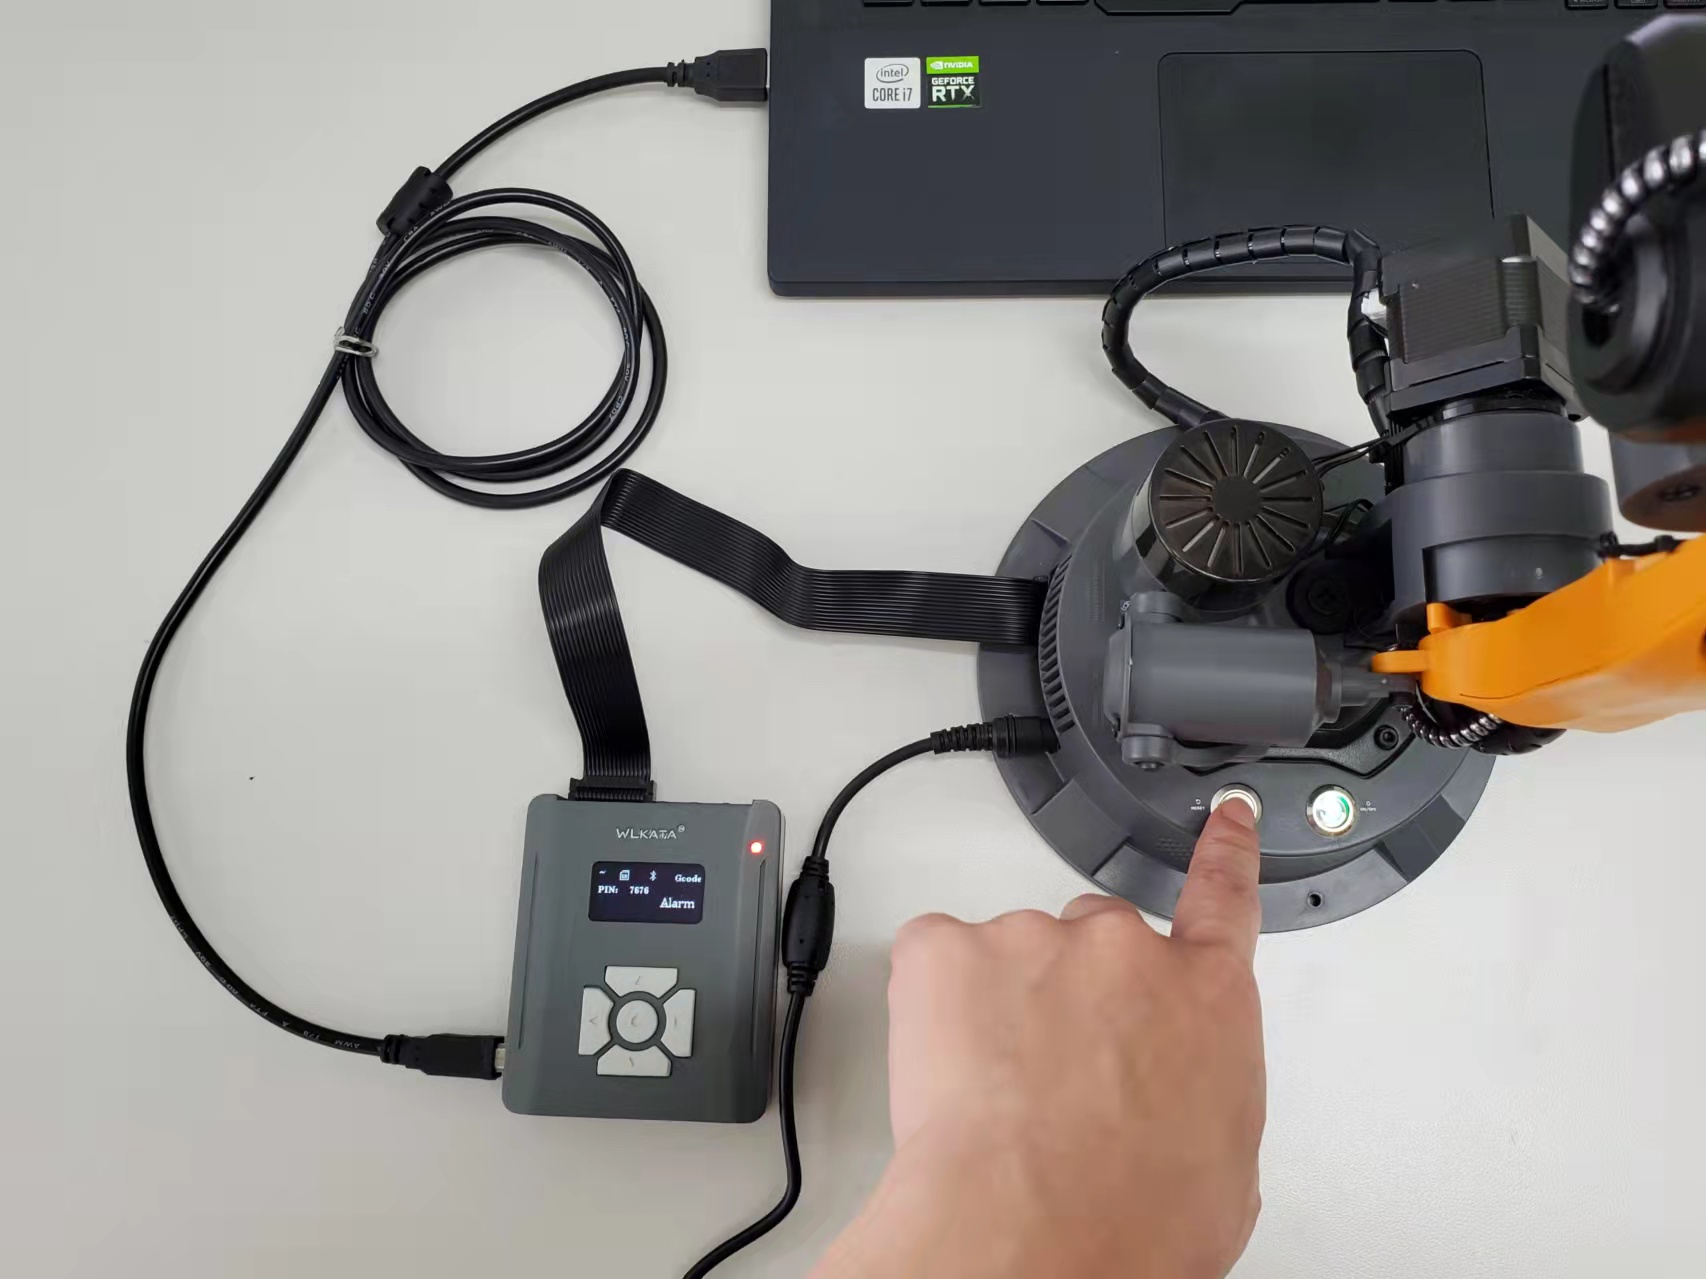
\includegraphics[width=10cm]{image/hardware_setup.jpg}
  \caption*{Powering on the Mirobot. The power button is to the right of the one the person above is pressing.}
%   \label{fig:galaxy}
\end{figure}

\paragraph{1D.} Check connection.
\begin{enumerate} %[(i)]
    \item Open WLKATA Studio.
    \item If the upper left corner of the WLKATA Studio interface displays CONNECTED, you are successfully connected. Otherwise, you may need to change the COM setting (\href{https://document.wlkata.com/?doc=/wlkata-mirobot-user-manual/12-quick-start-guide-of-mirobot/#header-three-6hmdl}{more details}).
    \item  When the robotic arm is powered on, or when the serial port connection is first established, each axis of the robotic arm is locked. To unlock the axes and perform any operations, the robotic must be homed. Click the HOMING button in the WLKATA Studio. Wait for the manipulator to be homed. Please attach a photo of your robot after the homing operation. It should look like the one below.
\end{enumerate}
\begin{figure}[H]
  \centering
  \vspace*{-0.0 in}
  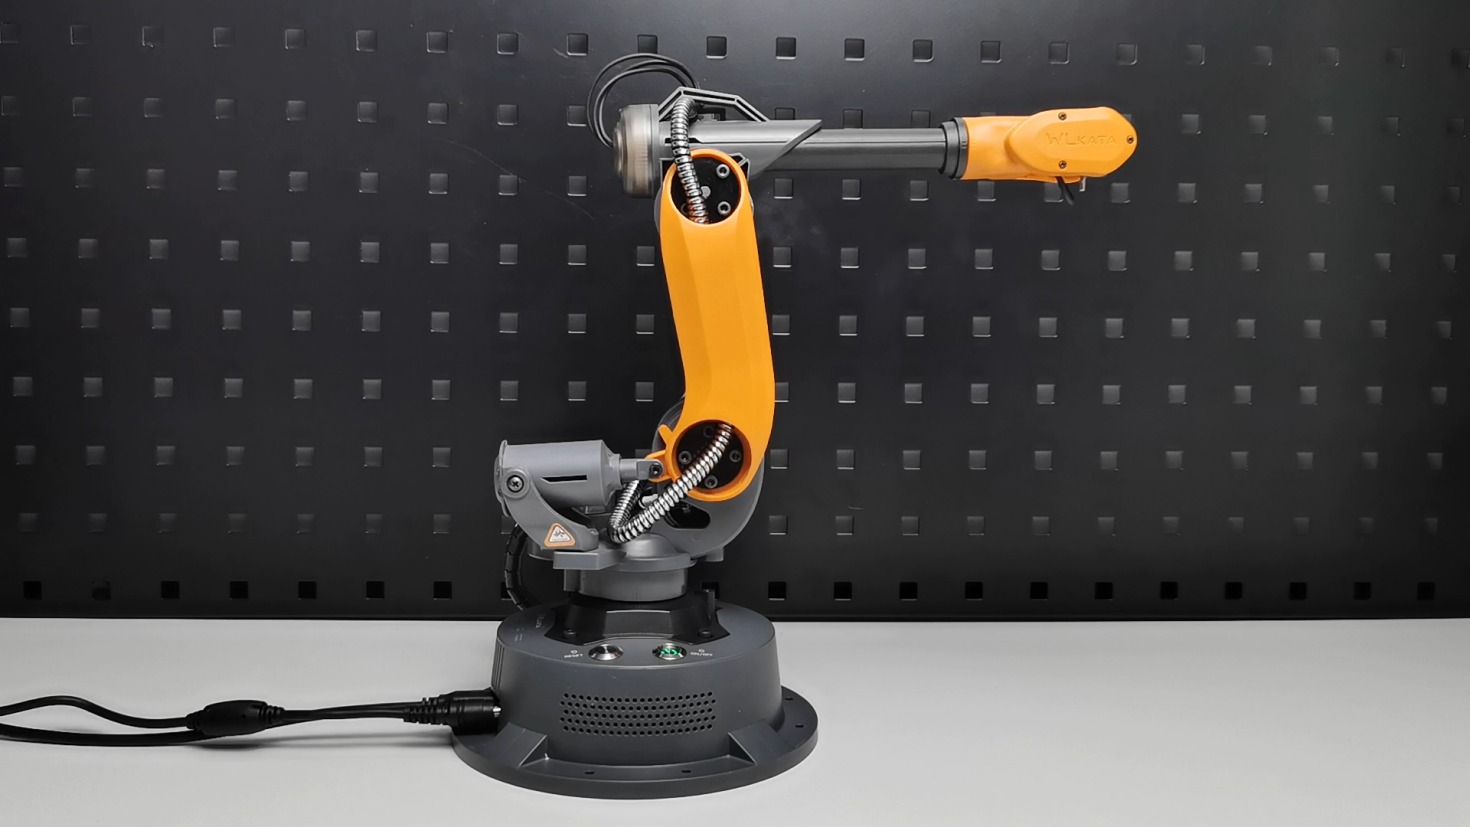
\includegraphics[width=10cm]{image/post_homing.png}
  \caption*{The correct position of the manipulator after a successful HOMING action}
%   \label{fig:galaxy}
\end{figure}


\paragraph{1E.} Inverse Kinematics.\\
\noindent Set the robot mode to \textbf{COORD MODE} (\href{https://document.wlkata.com/?doc=/wlkata-mirobot-user-manual/12-quick-start-guide-of-mirobot/\#header-three-2mfvd}{more details}) within the studio to move the robot arm to a target position marked \texttt{TARGET A} on the mat.
Submit photo result in the space provided.



\paragraph{1F.} Forward Kinematics.\\
\noindent Set the robot to \textbf{JOINT MODE} (\href{https://document.wlkata.com/?doc=/wlkata-mirobot-user-manual/12-quick-start-guide-of-mirobot/\#header-three-2mfvd}{more details}) within the studio to move the robot arm to a target position marked \texttt{TARGET B} on the mat. Submit photo result in the space provided.
%%%%%% DON'T MODIFY UNTIL HERE

\newpage

\paragraph{Answers.}
Please do not exceed the height provided for each answer image.
%%%%%% YOU ANSWER STARTS HERE

% NOTE: MAKE SURE YOU DON'T CHANGE THE HEIGHT OF IMAGES
% NOTE: MAKE SURE TO REMOVE THE 'draft' OPTION FOR includegraphics BELOW. OTHERWISE, YOU WILL NOT SEE YOUR IMAGES.

\paragraph{1A. Robot Use Agreement}
\begin{center}
    \includegraphics[draft,height=2.5in]{YOUR\_ANSWER.png}
\end{center}

\paragraph{1B. WLKATA Studio}
\begin{center}
    \includegraphics[draft,height=2.5in]{YOUR\_ANSWER.png}
\end{center}

\newpage
\paragraph{1C. Set up hardware}
\begin{center}
    \includegraphics[draft,height=2.5in]{YOUR\_ANSWER.png}
\end{center}

\paragraph{1D. Check Connection}
\begin{center}
    \includegraphics[draft,height=2.5in]{YOUR\_ANSWER.png}
\end{center}

\newpage
\paragraph{1E. Inverse Kinematics}
\begin{center}
    \includegraphics[draft,height=2.5in]{YOUR\_ANSWER.png}
\end{center}

\paragraph{1F. Forward Kinematics}
\begin{center}
    \includegraphics[draft,height=2.5in]{YOUR\_ANSWER.png}
\end{center}

\newpage

\paragraph{Additional Space.}
Please do not exceed this page for this question.
%%%%%% YOU ANSWER ENDS HERE

%%%%%% DON'T MODIFY STARTING HERE
\newpage
\section*{2. Python API}

For this section, you may reference the template code or the \href{https://document.wlkata.com/?doc=/wlkata-mirobot-resources-for-education/python-sdk/}{documentation}. This \href{https://docs.google.com/document/d/1Jh17WoaQvjzbp1AMjOTzPfXSAxNnE87V8AEH1H-iLk8/edit?usp=sharing}{handbook} may also be useful for additional information.
For all subsequent exercises, we will create a Python virtual environment using \href{https://www.anaconda.com/products/individual}{Anaconda}.
Please install Anaconda as instructed in the above link, then create a new environment:
%
\begin{verbatim}
    conda create -n 52-O python=3.8
\end{verbatim}

Then activate this virtual environment. You must do this for all subsequent exercises even if not instructed.
\begin{verbatim}
    conda activate 52-O
\end{verbatim}

\paragraph{2A.} Install Python SDK: \texttt{pip install wlkata-mirobot-python}. Attach at screenshot that shows successful completion in the space provided.

\paragraph{2B.} Create robot arm object and home.
Attach a screenshot of successful command execution.
\begin{enumerate} %[(i)]
    \item \texttt{arm = WlkataMirobot(portname=``your port name")}
    \item \texttt{arm.home()}
\end{enumerate}

\paragraph{2C.} Replicate \textbf{1E} and \textbf{1F} using the Python API.
Consult the documentation to figure out the values for \texttt{joint\_angles}, \texttt{x, y, z}, etc.
Submit photo result and include your code in the space provided.
\begin{itemize}
    \item \texttt{def set\_joint\_angle(self, joint\_angles, is\_relative=False, speed=None, wait\_ok=None)}
    \item \texttt{def set\_tool\_pose(self, x=None, y=None, z=None, roll=0.0, pitch=0.0, yaw=0.0,  mode='p2p', speed=None, is\_relative=False, wait\_ok=True)}
\end{itemize}



\paragraph{2D} Utilize the below 4 interpolation functions to make the robot go from \texttt{TARGET A} to \texttt{TARGET B} on the mat.
Submit photo result of the arm in \textbf{both} targets in the space provided.
Please also include your code where appropriate.
% TODO
\begin{itemize}
    \item Point2Point: \texttt{def p2p\_interpolation(self, x=None, y=None, z=None, a=None, b=None, c=None, speed=None, is\_relative=False, wait\_ok=None)}
    \item Linear: \texttt{def linear\_interpolation(self, x=None, y=None, z=None, a=None, b=None, c=None, speed=None, is\_relative=False, wait\_ok=None)}
    \item Door: \texttt{def door\_interpolation(self, x=None, y=None, z=None, a=None, b=None, c=None, speed=None, is\_relative=False, wait\_ok=None)}
    \item Circular: \texttt{def circular\_interpolation(self, ex, ey, radius, is\_cw=True, speed=None, wait\_ok=None)}
\end{itemize}
%%%%%% DON'T MODIFY UNTIL HERE

\paragraph{Answers.}
Please do not exceed the height provided for each answer image.
%%%%%% YOU ANSWER STARTS HERE

% NOTE: MAKE SURE YOU DON'T CHANGE THE HEIGHT OF IMAGES
% NOTE: MAKE SURE TO REMOVE THE 'draft' OPTION FOR includegraphics BELOW. OTHERWISE, YOU WILL NOT SEE YOUR IMAGES.

\paragraph{2A. Install Python SDK}
\begin{center}
    \includegraphics[draft,height=2.5in]{YOUR\_ANSWER.png}
\end{center}

\paragraph{2B. Create Python Object and Home}
\begin{center}
    \includegraphics[draft,height=2.5in]{YOUR\_ANSWER.png}
\end{center}

\newpage
\paragraph{2C. IK / FK using Python}
Include your code also.

\begin{figure}[hb!]
     \centering
    \begin{subfigure}[b]{0.3\textwidth}
        \includegraphics[draft,height=2.5in]{YOUR\_ANSWER.png}
         \caption*{Inverse Kinematics to \texttt{TARGET A}}
     \end{subfigure}
     %
     \hfill
     %
     \begin{subfigure}[b]{0.3\textwidth}
        \includegraphics[draft,height=2.5in]{YOUR\_ANSWER.png}
         \caption*{Forward Kinematics to \texttt{TARGET A}}
     \end{subfigure}
    \caption*{Answer for 2C.}
\end{figure}

\begin{minted}{python}
    var = 'YOU CODE GOES HERE'
\end{minted}

\newpage
\paragraph{2D. Interpolation}
Include your code also.

\begin{figure}[hb!]
     \centering
    \begin{subfigure}[b]{0.3\textwidth}
        \includegraphics[draft,height=2.5in]{YOUR\_ANSWER.png}
         \caption*{Point2Point: \texttt{TARGET A}}
     \end{subfigure}
     %
     \hfill
     %
     \begin{subfigure}[b]{0.3\textwidth}
        \includegraphics[draft,height=2.5in]{YOUR\_ANSWER.png}
         \caption*{Point2Point: \texttt{TARGET B}}
     \end{subfigure}
    \caption*{Answer for 2C.}
\end{figure}
%
\begin{minted}{python}
    var = 'YOU CODE GOES HERE'
\end{minted}

\newpage
\begin{figure}[hb!]
     \centering
    \begin{subfigure}[b]{0.3\textwidth}
        \includegraphics[draft,height=2.5in]{YOUR\_ANSWER.png}
         \caption*{Linear: \texttt{TARGET A}}
     \end{subfigure}
     %
     \hfill
     %
     \begin{subfigure}[b]{0.3\textwidth}
        \includegraphics[draft,height=2.5in]{YOUR\_ANSWER.png}
         \caption*{Linear: \texttt{TARGET B}}
     \end{subfigure}
    \caption*{Answer for 2C.}
\end{figure}
%
\begin{minted}{python}
    var = 'YOU CODE GOES HERE'
\end{minted}

\newpage
\begin{figure}[hb!]
     \centering
    \begin{subfigure}[b]{0.3\textwidth}
        \includegraphics[draft,height=2.5in]{YOUR\_ANSWER.png}
         \caption*{Door: \texttt{TARGET A}}
     \end{subfigure}
     %
     \hfill
     %
     \begin{subfigure}[b]{0.3\textwidth}
        \includegraphics[draft,height=2.5in]{YOUR\_ANSWER.png}
         \caption*{Door: \texttt{TARGET B}}
     \end{subfigure}
    \caption*{Answer for 2C.}
\end{figure}
%
\begin{minted}{python}
    var = 'YOU CODE GOES HERE'
\end{minted}

\newpage
\begin{figure}[hb!]
     \centering
    \begin{subfigure}[b]{0.3\textwidth}
        \includegraphics[draft,height=2.5in]{YOUR\_ANSWER.png}
         \caption*{Circular: \texttt{TARGET A}}
     \end{subfigure}
     %
     \hfill
     %
     \begin{subfigure}[b]{0.3\textwidth}
        \includegraphics[draft,height=2.5in]{YOUR\_ANSWER.png}
         \caption*{Circular: \texttt{TARGET B}}
     \end{subfigure}
    \caption*{Answer for 2C.}
\end{figure}
%
\begin{minted}{python}
    var = 'YOU CODE GOES HERE'
\end{minted}

\newpage

\paragraph{Additional Space.}
Please do not exceed this page for this question.
%%%%%% YOU ANSWER ENDS HERE

%%%%%% DON'T MODIFY STARTING HERE
\newpage
\section*{3. End Effectors}

For this section, you may reference the template code or the \href{https://document.wlkata.com/?doc=/wlkata-mirobot-resources-for-education/python-sdk/#header-step-8npsc}{documentation}.
You will perform the same task using 3 different end effectors.
%
\begin{figure}[h!]
    \centering
    \begin{subfigure}[b]{0.27\textwidth}
        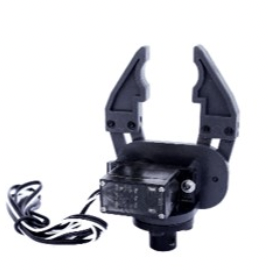
\includegraphics[width=2cm]{image/gripper.png}
        \caption*{Gripper}
    \end{subfigure}
    \hfill
    \begin{subfigure}[b]{0.27\textwidth}
        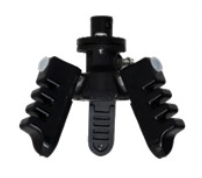
\includegraphics[width=2cm]{image/3finger.png}
        \caption*{Flexible Claw}
    \end{subfigure}
    \hfill
    \begin{subfigure}[b]{0.27\textwidth}
    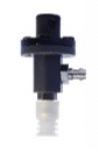
\includegraphics[width=1.2cm]{image/suction cup.png}
    \caption*{Suction Cup}
    \end{subfigure}
    \caption*{Types of end effectors.}
\end{figure}

\paragraph{3A.} Change end effectors. Attach a picture of each after successfully attaching each end effector.
\begin{enumerate} %[(i)]
    \item Power off the robot
    \item For the gripper, connect it to the correct port on the Multifunctional Extender Box (MEB). For the claw and suction cup, connect the pneumatic pump to the MEB.
    Make sure to connect the pump to the gripper as needed.
\begin{figure}[H]
  \centering
  \vspace*{-0.0 in}
  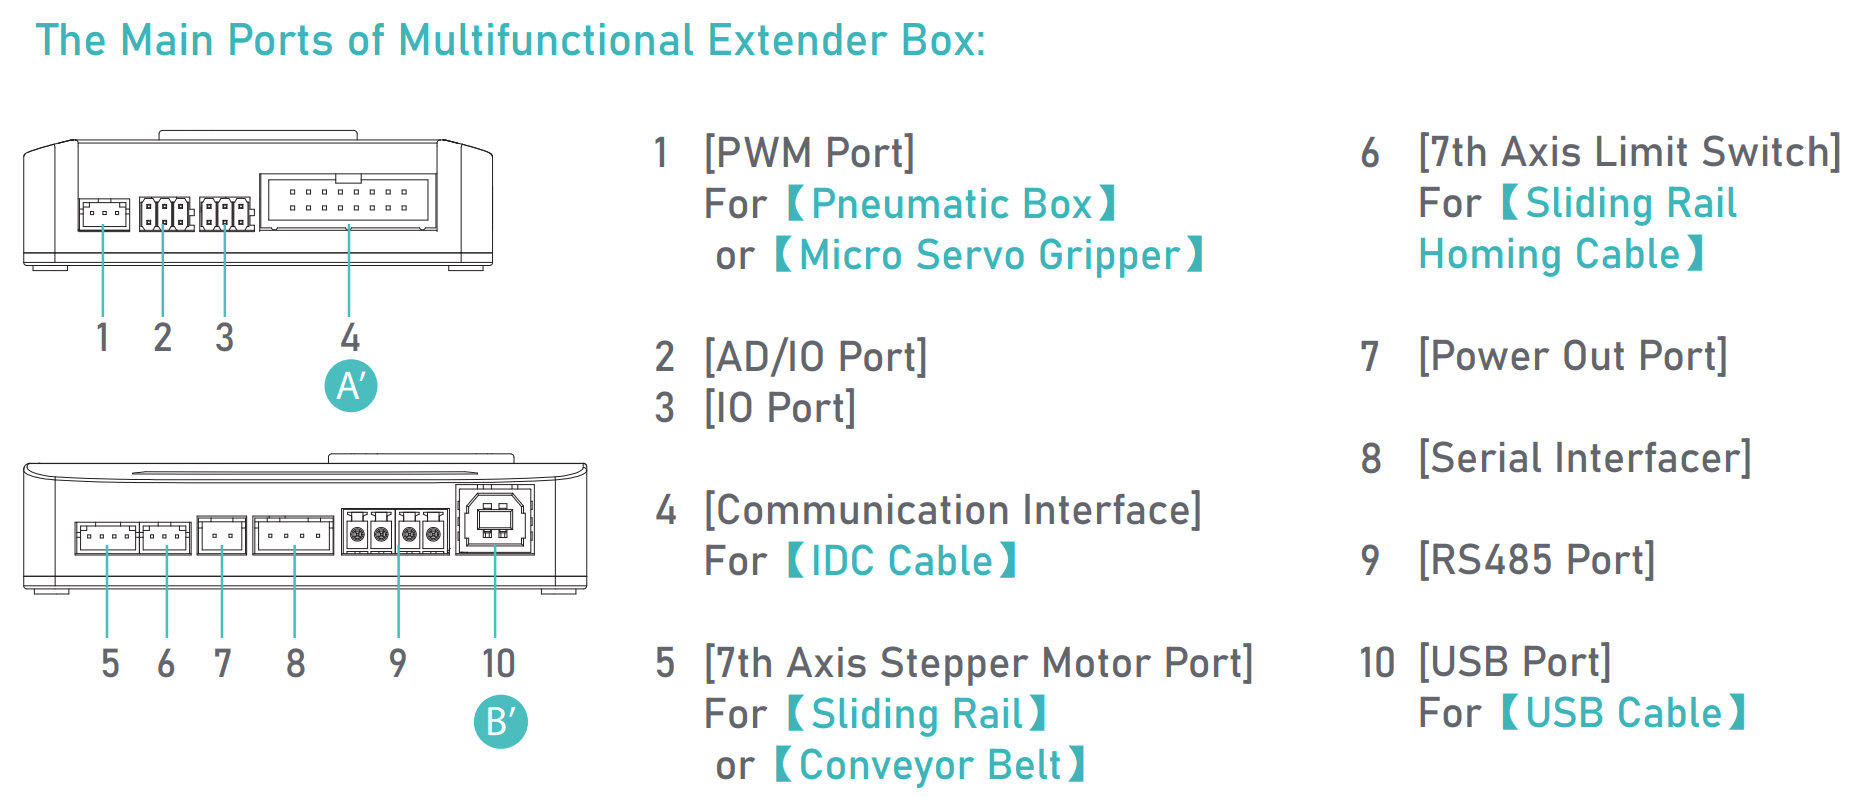
\includegraphics[width=10cm]{image/endeffectors.png}
  \caption*{Use port 1 to connect the end effectors}
  \end{figure}
    \item Connect the MEB to the robot.
    \item Screw on the end effector (an Allen wrench is the the tool box).
    Be careful to connect all wires before screwing on the end effector.
    \begin{figure}[H]
   \centering
    \vspace*{-0.0 in}
    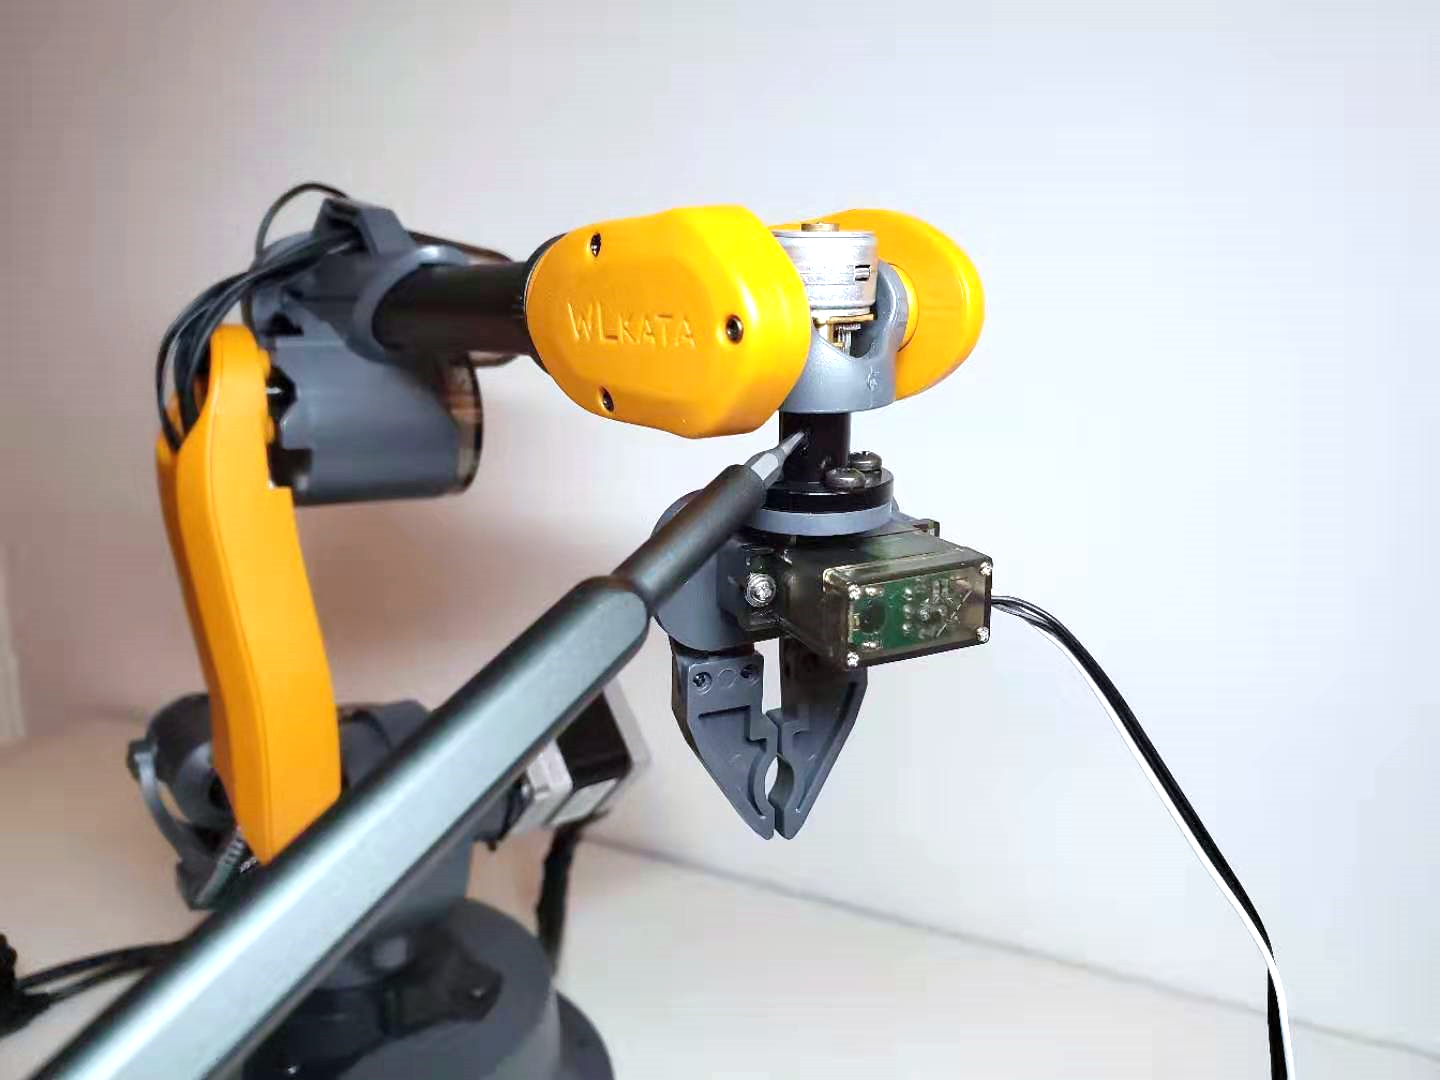
\includegraphics[width=10cm]{image/screwingendeffector.png}
    \caption*{How to screw on the end effector. Use the Allen wrench in the toolbox.}
\end{figure}
\end{enumerate}

\paragraph{3B.} Use the gripper (2 finger) to grab any toy block from the table. Submit photo result of the robot successfully lifting a block in the space provided.
    \begin{enumerate}
        \item Complete the task using the studio software
        \item Complete the task using Python API
        \begin{itemize}
        \item \texttt{from wlkata\_mirobot import WlkataMirobotTool}
        \item \texttt{arm.set\_tool\_type(WlkataMirobotTool.GRIPPER)}
        \item \texttt{arm.gripper\_open()}
        \item \texttt{arm.gripper\_close()}
        \item \texttt{arm.set\_gripper\_spacing(spacing\_mm)}
        \end{itemize}
    \end{enumerate}
    
\paragraph{3C.} Use the flexible claw (3 finger soft gripper) to grab any block from the table. Submit photo result of the robot successfully lifting a block in the space provided.

    
    \begin{enumerate}
        \item Complete the task using the studio software
        \item Complete the task using Python API
        \begin{itemize}
        \item For flexible claws, air pump suction represents opening and blowing represents closing.
        \item \texttt{arm.set\_tool\_type(WlkataMirobotTool.FLEXIBLE\_CLAW)}
        \item \texttt{arm.pump\_suction()}
        \item \texttt{arm.pump\_blowing()}
        \end{itemize}
    \end{enumerate}

\paragraph{3D.} Use the suction cup to grab any block from the table. Submit photo result of the robot successfully lifting a block in the space provided.

    \begin{enumerate}
        \item Complete the task using the studio software
        \item Complete the task using Python API
        \begin{itemize}
        \item \texttt{arm.set\_tool\_type(WlkataMirobotTool.FLEXIBLE\_CLAW)}
        \item \texttt{arm.pump\_suction()}
        \item \texttt{arm.pump\_blowing()}
        \end{itemize}
    \end{enumerate}
     \begin{figure}[H]
   \centering
    \vspace*{-0.0 in}
    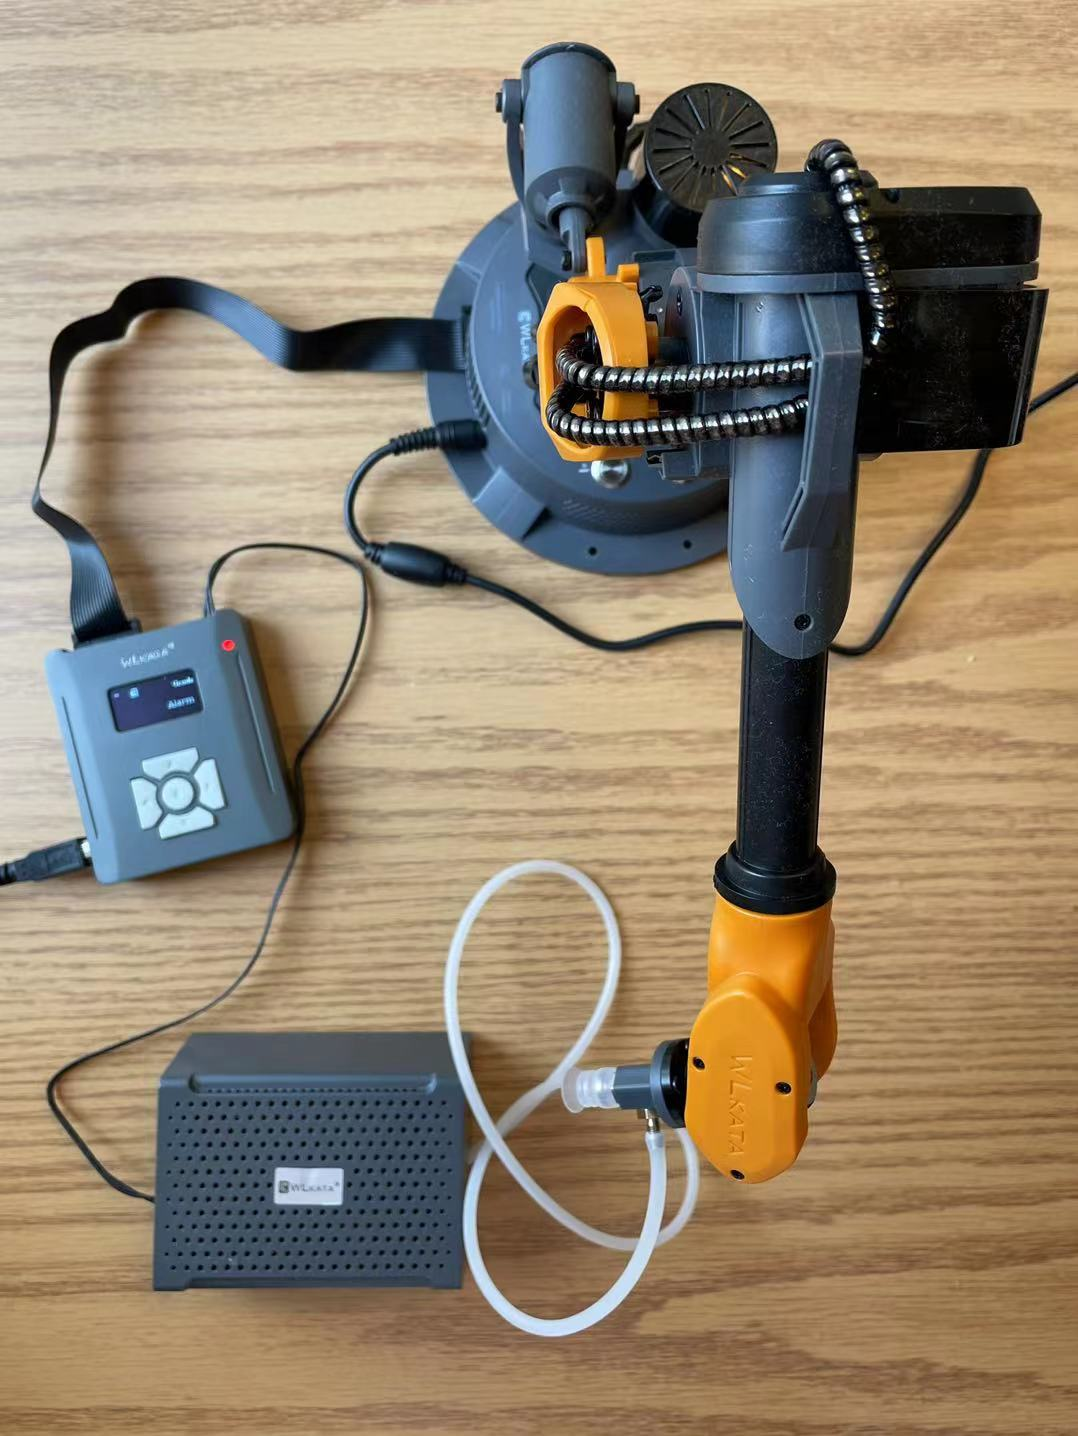
\includegraphics[width=10cm]{image/vacuumsetup.jpg}
    \caption*{Image showing how to use the pneumatic pump.}
\end{figure}
%%%%%% DON'T MODIFY UNTIL HERE

\newpage
\paragraph{Answers.}
Please do not exceed the height provided for each answer image.
%%%%%% YOU ANSWER STARTS HERE

% NOTE: MAKE SURE YOU DON'T CHANGE THE HEIGHT OF IMAGES
% NOTE: MAKE SURE TO REMOVE THE 'draft' OPTION FOR includegraphics BELOW. OTHERWISE, YOU WILL NOT SEE YOUR IMAGES.

\paragraph{3A. Change End Effectors}
%
\begin{figure}[h!]
    \centering
    \begin{subfigure}[b]{0.3\textwidth}
        \includegraphics[draft,height=2.5in]{YOUR\_ANSWER.png}
         \caption*{Mirobot with Gripper.}
     \end{subfigure}
     %
     \hfill
     %
     \begin{subfigure}[b]{0.3\textwidth}
        \includegraphics[draft,height=2.5in]{YOUR\_ANSWER.png}
         \caption*{Mirobot with Flexible Claw.}
     \end{subfigure}
     %
     \hfill
     %
     \begin{subfigure}[b]{0.3\textwidth}
        \includegraphics[draft,height=2.5in]{YOUR\_ANSWER.png}
         \caption*{Mirobot with Suction Cup.}
     \end{subfigure}     
    \caption*{Answer for 3A.}
\end{figure}
%
\begin{minted}{python}
    var = 'YOU CODE GOES HERE'
\end{minted}

\newpage
\paragraph{3B. Using Gripper.}
\begin{figure}
    \centering
    \begin{subfigure}[b]{0.3\textwidth}
        \includegraphics[draft,height=2.5in]{YOUR\_ANSWER.png}
         \caption*{Gripper lifting a block (WLKATA Studio).}
     \end{subfigure}
     %
     \hfill
     %
     \begin{subfigure}[b]{0.3\textwidth}
        \includegraphics[draft,height=2.5in]{YOUR\_ANSWER.png}
         \caption*{Gripper lifting a block (Python).}
     \end{subfigure}
    \caption*{Answer for 3B.}
\end{figure}
%
\begin{minted}{python}
    var = 'YOU CODE GOES HERE'
\end{minted}


\newpage
\paragraph{3C. Using Flexible Claw.}
\begin{figure}
    \centering
    \begin{subfigure}[b]{0.3\textwidth}
        \includegraphics[draft,height=2.5in]{YOUR\_ANSWER.png}
         \caption*{Flexible Claw lifting a block (WLKATA Studio).}
     \end{subfigure}
     %
     \hfill
     %
     \begin{subfigure}[b]{0.3\textwidth}
        \includegraphics[draft,height=2.5in]{YOUR\_ANSWER.png}
         \caption*{Flexible Claw lifting a block (Python).}
     \end{subfigure}
    \caption*{Answer for 3C.}
\end{figure}
%
\begin{minted}{python}
    var = 'YOU CODE GOES HERE'
\end{minted}


\newpage
\paragraph{3D. Using Suction Cup.}
\begin{figure}
    \centering
    \begin{subfigure}[b]{0.3\textwidth}
        \includegraphics[draft,height=2.5in]{YOUR\_ANSWER.png}
         \caption*{Suction Cup lifting a block (WLKATA Studio).}
     \end{subfigure}
     %
     \hfill
     %
     \begin{subfigure}[b]{0.3\textwidth}
        \includegraphics[draft,height=2.5in]{YOUR\_ANSWER.png}
         \caption*{Suction Cup lifting a block (Python).}
     \end{subfigure}
    \caption*{Answer for 3D.}
\end{figure}
%
\begin{minted}{python}
    var = 'YOU CODE GOES HERE'
\end{minted}


\newpage
\paragraph{Additional Space.}
Please do not exceed this page for this question.
%%%%%% YOU ANSWER ENDS HERE

%%%%%% DON'T MODIFY STARTING HERE
\newpage
\section*{4.ROS Integration}

\paragraph{4A.} Install ROS kinetic \href{http://wiki.ros.org/Installation}{here}. Be sure to select the ``kinetic" tab after clicking on the platform option.
Make sure to activate the \texttt{52-O} conda environment we created earlier.
Attach screenshot of successful installation.

\paragraph{4B.} Install relevant ROS packages. Make sure to activate the \texttt{52-O} conda environment we created earlier.
Attach screenshot of successful installation.
\begin{itemize}
    \item \texttt{ros-kinetic-serial}
    \item \texttt{ros-kinetic-ros-control }
    \item \texttt{ros-kinetic-ros-controllers }
    \item \texttt{ros-kinetic-moveit }
    \item \texttt{ros-kinetic-gazebo-ros-pkgs }
    \item \texttt{ros-kinetic-gazebo-ros-control}
\end{itemize}

\paragraph{4C.} Replicate \textbf{1E} and \textbf{1F} using ROS. Reference the \href{https://document.wlkata.com/?doc=/wlkata-mirobot-resources-for-education/ros/ }{wlkata documentation} and \href {https://github.com/wlkata/RosForMirobot-master}{github repo}. Submit photo result in the space provided.
%%%%%% DON'T MODIFY UNTIL HERE
 
\newpage
\paragraph{Answers.}
Please do not exceed the height provided for each answer image.
%%%%%% YOU ANSWER STARTS HERE

% NOTE: MAKE SURE YOU DON'T CHANGE THE HEIGHT OF IMAGES
% NOTE: MAKE SURE TO REMOVE THE 'draft' OPTION FOR includegraphics BELOW. OTHERWISE, YOU WILL NOT SEE YOUR IMAGES.

\paragraph{4A. Install ROS kinetic.}
\begin{center}
    \includegraphics[draft,height=2.5in]{YOUR\_ANSWER.png}
\end{center}

\paragraph{4B. Install ROS Packages.}
\begin{center}
    \includegraphics[draft,height=2.5in]{YOUR\_ANSWER.png}
\end{center}

\newpage
\paragraph{4C. Inverse Kinematics}
\begin{center}
    \includegraphics[draft,height=2.5in]{YOUR\_ANSWER.png}
\end{center}

\paragraph{4C. Forward Kinematics}
\begin{center}
    \includegraphics[draft,height=2.5in]{YOUR\_ANSWER.png}
\end{center}

\newpage
\paragraph{Additional Space.}
Please do not exceed this page for this question.
%%%%%% YOU ANSWER ENDS HERE

%%%%%% DON'T MODIFY STARTING HERE
\newpage
\section*{5. Cameras \& Mirobot}

In addition to the Mirobot, you will also work with the RealSense D400 series of sensors.
These sensors have an RGB camera as well as a 3D depth sensor.
In this exercise you will learn how to interface with these cameras and calibrate them relative to the robot.

\paragraph{5A.} Install OpenCV and RealSense API as instructed below. Attach a final screenshot of your prompt after step 3.
\begin{enumerate}
    \item Activate your conda environment: \texttt{conda activate 52-O}
    \item Install OpenCV: \texttt{conda install -c conda-forge opencv}
    \item Install the \href{https://github.com/IntelRealSense/librealsense/tree/master/wrappers/python#installation}{\texttt{pyrealsense2}} library: \texttt{pip install pyrealsense2}
\end{enumerate}

\paragraph{5B.} Connect the camera to your machine.\\

The camera uses a USB 3 connection and a USB-C connector. Please connect \textbf{both} the camera and the robot into your machine.
Please use the provided USB hub, if needed.
Attach a photo of the camera and robot attached to your machine.

\paragraph{5C.} Visualize camera output using OpenCV.

\begin{enumerate}
    \item Run the Python script \texttt{code/q5c\_1.py}. Attach a screenshot of what you see when you run this code.
    \item Run the Python script \texttt{code/q5c\_2.py}. Attach a screenshot of what you see when you run this code.
\end{enumerate}

\paragraph{5D.} Camera calibration.
Follow this \href{https://docs.opencv.org/3.4/dc/dbb/tutorial_py_calibration.html}{tutorial} to understand camera intrinsics and extrinsics calibration.
Use the \texttt{calibrateCamera} function in OpenCV and implement calibration of both intrinsics and extrinsics.
Please attach your code and the intrinsics matrix (\texttt{cameraMatrix}) for the RGB camera in Intel RealSense.

You may want to combine code from 5C for this part.
A printed 9x6 checkerboard pattern is available in your workspace.
You can also find it \href{https://drive.google.com/file/d/1Hk-U4xiAmZnrf3qGziQWBW7YbEMFTWgY/view?usp=sharing}{here}.
%%%%%% DON'T MODIFY UNTIL HERE
 
\newpage
\paragraph{Answers.}
Please do not exceed the height provided for each answer image.
%%%%%% YOU ANSWER STARTS HERE

% NOTE: MAKE SURE YOU DON'T CHANGE THE HEIGHT OF IMAGES
% NOTE: MAKE SURE TO REMOVE THE 'draft' OPTION FOR includegraphics BELOW. OTHERWISE, YOU WILL NOT SEE YOUR IMAGES.

\paragraph{5A. Install OpenCV and RealSense API.}
\begin{center}
    \includegraphics[draft,height=2.5in]{YOUR\_ANSWER.png}
\end{center}

\paragraph{5B. Connect Camera to your machine.}
\begin{center}
    \includegraphics[draft,height=2.5in]{YOUR\_ANSWER.png}
\end{center}

\newpage
\paragraph{5C. Visualize using OpenCV.}
\begin{center}
    \includegraphics[draft,height=2.5in]{YOUR\_ANSWER.png}
\end{center}

\paragraph{5D. Camera Calibration.}
%
\begin{minted}{python}
    var = 'YOU CODE GOES HERE'
\end{minted}

Please also report the matrix stored in the \texttt{cameraMatrix} return variable of the \texttt{calibrateCamera} function.


\newpage
\paragraph{Additional Space.}
Please do not exceed this page for this question.
%%%%%% YOU ANSWER ENDS HERE

%%%%%%%%%%%%%%%%%%%%%%%%%%%%%%%%%%%

% Please leave the pagebreak
%% any suggestions for more?
\pagebreak
\section*{Feedback}
Please help us make the course better. If you have any feedback for this assignment, we'd love to hear it!

\end{document}
